\documentclass[11pt,numbers=noenddot,svgnames]{scrbook}
\usepackage[top=1in, left=1in, right=1in, bottom=1in]{geometry}
\usepackage{evanbook}
\usepackage{pgfplots}
\usepackage{float}
\DeclareMathOperator{\Deg}{deg}
\begin{document}

\chapter{Polynomials}

\begin{definition}
    A Polynomial $P(x)$ is an one variable expression or function of the form
    \[
        P(x) = \sum_{i=0}^{n} a_{i}x^{i} = a_{n}x^{n} + a_{n-1}x^{n-1} + \cdots +a_{1}x + a_{0}
    \]
    where $a_{0},a_{1}, \cdots, a_{n}$ are constants and $n \in \mathbb{N}$. The constants $a_{i}$ are called the 
    \textit{coefficients} of the polynomial. We will denote $A[x]$ as the set of all polynomials with $a_{i} \in A$. If 
    $n\neq 0$ then $n$ is called the \textit{degree} of the polynomial $P(x)$ and write $\Deg P(x)=n$. 
    If $a_{n} = 1$ then we say that the polynomial is \textit{monic}. \\
    $r$ is called a \textit{root} of the polynomial $P(x)$ if and only if $P(r)=0$.
\end{definition}

\section{Division Algorithm}

\begin{theorem}[The Division Algorithm]\label{thm:division-algorithm}
    Given two polynomial $A(x)$ and $B(x)$ there exists unique polynomials $Q(x)$ and $R(x)$ with $\Deg R(x) < \Deg B(x)$ 
    such that,
    \[
        A(x) = Q(x)B(x) + R(x)
    \]
    The polynomials $Q(x)$ and $R(x)$ are known as the \textit{quotient} and the \textit{remainder}, respectively. If the 
    remainder $R(x)=0$ then we say that $B(x)$ divides $A(x)$ and write $B(x) \mid A(x)$.
\end{theorem}

For example, if $B(x)= x^{2}-x+1$ and $A(x)=x^{5}+x^{3}+2x$ then,
\[
    x^{5}+x^{3}+2x = \left(x^{3}+x^{2}+x\right) \left(x^{2}-x+1\right) +x
\]
In this example, the remainder $R(x)=x$ and the quotient $Q(x)=x^{3}+x^{2}+x$. \\
Suppose $B(x)$ is a polynomial of degree $n\geq 1$ and let $A(x)=x-z$ be linear polynomial. Now from 
\hyperref[thm:division-algorithm]{Theorem \ref{thm:division-algorithm}} we know that there exists polynomials 
$Q(x)$ and $R(x)$ with $\Deg R(x) < 1$ such that,
\[
    B(x) = A(x)Q(x) + R(x)
\]
Since $0 \leq \Deg R(x) < 1$, $R(x)$ must be a constant polynomial, we can assume $R(x)=r$ where $r \in \mathbb{R}$. 
Therefore,
\begin{align*}
    B(x) &= A(x)Q(x) + R(x) \\
         &= (x - z)Q(x) + r
\end{align*}
Now if $r=0$ then,
\[
    B(x) = (x-z)Q(x) \implies B\left(z\right) = 0
\]
Now if $B\left(z\right)=0$ that is if $z$ is a root of the polynomial $B(x)$ then,
\[
    B\left(z\right) = \left(z - z\right)Q(x) + r \implies B\left(z\right)=r \implies 
    r=0
\]
Therefore we have proved the following theorem.
\begin{theorem}[Factor Theorem]\label{thm:factor-theorem}
    The real number $z$ will be a root of the polynomial $P(x)$ if and only if $P(x)$ is divisible by $x-z$.
\end{theorem}
\begin{corollary}
    The number $-\frac{b}{a}$ where $a, b\in \mathbb{R}$ will be a root of the polynomial $P(x)$ if and only if the 
    polynomial $P(x)$ is divisible by $ax+b$.
\end{corollary}
If $P(x)$ has the root $z$ then the \hyperref[thm:factor-theorem]{Factor Theorem} guarantees that there exists a polynomial 
$Q_{0}(x)$ such that,
\[
    P(x) = \left(x - z\right)Q_{0}(x)
\]
Now if,
\[
    P(x) = \left(x-z\right)^{m}Q(x)
\]
then we say that $z$ is root of $P(x)$ of \textit{multiplicity} $m$.

\section{The Fundamental Theorem of Algebra}

\begin{theorem}[The Fundamental Theorem of Algebra]\label{thm:fta}
    The Fundamental Theorem of Algebra states that, every polynomial $P(x)$ in $\mathbb{C}[x]$ has at least 
    one root in $\mathbb{C}$
\end{theorem}
\begin{corollary}
    If $P(x) = a_{n}x^{n} + a_{n-1}x^{n-1} + \cdots + a_{1}x + a_{0}$ is a polynomial of degree $n$ then,
    \[
        P(x) = k(x - z_{1})(x - z_{2})\cdots (x - z_{n})
    \]
    where, $k = a_{n}$ and $z_{i} \in \mathbb{C}$. The numbers $z_{1},z_{2}\cdots z_{n}$ are not necessarily 
    distinct.
\end{corollary}
\section{Roots of Cubic Polynomials}

Finding the roots of a cubic polynomial is quite hard. So, we are going to first try to solve the cubic polynomial,
\[
    f(x) = x^{3} + px + q
\]
where $p, q \in \mathbb{R}$.
Setting $p=-3ab$ and $q = a^{3} + b^{3}$ we get,
\[
    f(x) = x^{3} + a^{3} + b^{3} - 3abx
\]
Now using the formula,
\[
    a^{3} + b^{3} + c^{3} - 3abc = (a+b+c)(a^{2} + b^{2} + c^{2} - ab - bc - ca)
\]
we get,
\[
    f(x) = (x+a+b)(x^{2} -(a+b)x + a^{2} + b^{2} - ab)
\]
Therefore the 3 roots of $f$ are,
\begin{align*}
    x_{1}        &= -a-b \\
    x_{2}, x_{3} &= \frac{a+b \pm \sqrt{a^{2} + b^{2} + 2ab - 4a^{2} - 4b^{2} + 4ab}}{2}\\
                 &= \frac{a+b \pm \sqrt{-3a^{2} -3b^{2} + 6ab}}{2} \\
                 &= \frac{a+b \pm \sqrt{-3(a-b)^{2}}}{2} \\
                 &= \frac{a+b \pm \sqrt{3}i(a-b)}{2} \\
                 &= \frac{(1 + \sqrt{3}i)a \pm (1 - \sqrt{3}i)b}{2} \\
                 &= \frac{1+\sqrt{3}i}{2}a \pm \frac{1-\sqrt{3}i}{2}b
\end{align*}

Now we have express the root in terms of $p, q$ that is, we have to express $a,b$ in terms of $p,q$. Now,

\begin{align*}
         & q = a^{3} + b^{3} \\
         & p = -3ab \\
\implies & a^{3}b^{3} = -\frac{p^{3}}{27}
\end{align*}

Let $u=a^{3}$ and $v=b^{3}$. Notice that $u$ and $v$ are the roots of the quadratic polynomial,
\[
    P(x) = x^{2} - (u+v)x + uv = x^{2} - q^{3}x -\frac{p^{3}}{27} 
\]

Using the quadratic equation we get,
\begin{align*}
    u,v &= \frac{q^{3} \pm \sqrt{q^{6} + \frac{4}{27}p^{3}}}{2} \\
    a,b &= \sqrt[3]{\frac{q^{3}}{2} \pm \frac{\sqrt{q^{6} + \frac{4}{27}p^{3}}}{2}}\\
        &= \sqrt[3]{\frac{q^{3}}{2} \pm \sqrt{\frac{q^{6}}{4} + \frac{p^{3}}{27}}}
\end{align*}

So let's now try to solve the cubic equation using the results we've got so far,
\[
    f(x) = x^{3} - x^{2} - 2x + 1
\]
First we have to use substitution to transform the polynomial into another polynomial of the form,
\[
    x^{3} + px + q
\]

Since every polynomial can be uniquely defined by its coefficients, we can associate or 
express a polynomial of degree $n$ by a unique point in $n+1$ dimensional space. 
For example we can express the polynomial,
\[
    (1) \cdot x^{3} + (-1) \cdot x^{2} + (-2) \cdot x + (1)
\]
as,
\[
    (1) \cdot x^{3} + (-1) \cdot x^{2} + (-2) \cdot x + (1) \rightarrow (1, -1, -2, 1)
\]
Likewise, the point $(5, -1, 0, 1)$ can be used to represent the polynomial,
\[
    (5, -1, 0, 1) \rightarrow 5x^{3} -x^{2} + 1
\]
Notice that,
\[
    (x_{3}, x_{2}, \cdots, x_{0}) + (y_{3}, y_{2}, \cdots, y_{0}) = (x_{3} + y_{3}, x_{2} + y_{2}, \cdots, x_{0} + y_{0})
\]

Say that there exists a polynomial $u(x) = (x+n)$ where $n \in \mathbb{C}$ such that,
\[
    x^{3} - x^{2} -2x + 1 = u(x)^{3} + pu(x) + q
\]
This equation can also be represented as,
\[
    (1, -1, -2, 1) = (1, 3n, 3n^{2}, n^{3}) + (0, 0, p, pn) + (0,0,0,q) \implies (1, -1, -2, 1) = (1, 3n, 3n^{2}+p, n^{3}+ pn + q)
\]
This gives us the system of equation,
\begin{align*}
   3n              &= -1 \\
   3n^{2} + p      &= -2 \\
    n^{3} + pn + q &= 1
\end{align*}

Therefore,
\begin{align*}
   n &= -\frac{1}{3} \\
   p &= -\frac{7}{3}\\
   q &=  \frac{7}{27}
\end{align*}

Thus,
\[
    x^{3} - x^{2} -2x +1 = \left(x - \frac{1}{3}\right)^{3} -\frac{7}{3}\left(x - \frac{1}{3}\right) +\frac{7}{27} \implies f(x) = g\left(x - \frac{1}{3}\right)
\]
where \[ g(x) = x^{3} - \frac{7}{3}x + \frac{7}{27} \]
Now we can use the results we've proved earlier to solve the polynomial $g(x)$. After that we add $\frac{1}{3}$ to the 3 roots 
of $g(x)$. The 3 numbers we will get by adding $\frac{1}{3}$ are the 3 roots of $f(x)$.

\section{Lagrange Interpolation}

\begin{theorem}[Lagrange Interpolation]\label{thm:lagrange-interpol}
    Let $\alpha_{0}, \alpha_{1},\cdots , \alpha_{n}$ be distinct real numbers and 
    $\beta_{0}, \beta_{1}, \cdots, \beta_{n}$ be another set of $n+1$ real numbers. 
    Then there exists a unique polynomial,
    \[
    P(x) = \sum_{i=0}^{n} \left( \prod_{\substack{j=0\\ j\neq i}}^{n} \frac{x - \alpha_{j}}{\alpha_{i} - \alpha_{j}} \right) \beta_{i}
    \]
    with $\Deg P(x) \leq n$ such that $P(\alpha_{k}) = \beta_{k}$ for all $0\leq k \leq n$.
\end{theorem}
\begin{proof}
    Let,
    \[
    D_{k}(x) = \prod_{\substack{j=0 \\ j\neq k}}^{n} \frac{x - \alpha_{j}}{\alpha_{k} - \alpha_{j}} = 
    \frac{(x-\alpha_{0})(x-\alpha_{1})\cdots (x - \alpha_{k-1})(x - \alpha_{k+1}) \cdots (x - \alpha_{n})}
         {(\alpha_{k}-\alpha_{0})(\alpha_{k}-\alpha_{1})\cdots (\alpha_{k} - \alpha_{k-1})(\alpha_{k} - \alpha_{k+1}) \cdots (\alpha_{k} - \alpha_{n})}
    \]
    If $x=\alpha_k$ then $D_k(x) = 1$ else if $x=\alpha_i$ where 
    $i \neq k$ then $D_k(x)=0$. Thus the polynomial,
    \[ P(x) = \sum_{k=0}^n D_k(x) \beta_k \]
    will be equal to $\beta_k$ for all $x=\alpha_k$. It is also clear that the 
    polynomial $P(x)$ has degree at most $n$ since $\Deg D_k(x)=n$ for all 
    $0 \leq k \leq n$. \\
    Now suppose that there exists two polynomials $P_1(x)$ and $P_2(x)$, with degree at 
    most $n$, such that,
    \[ P_1(\alpha_k) = P_2(\alpha_k) = \beta_k, \; 0\leq k \leq n\]
    Therefore the polynomial $Q(x) = P_1(x) - P_2(x)$ has $n+1$ distinct roots. 
    But that is impossible since we know that $\Deg Q(x) \leq n$ and 
    a polynomial of degree $n$ has at most $n$ distinct roots. This proves that 
    the polynomial $P(x)$ must be unique, that is, $P(x)$ is the only polynomial, with 
    degree at most $n$, such that, 
    $P(\alpha_k) = \beta_k$ for all $0 \leq k \leq n$
\end{proof}

\begin{figure}[H]
\centering
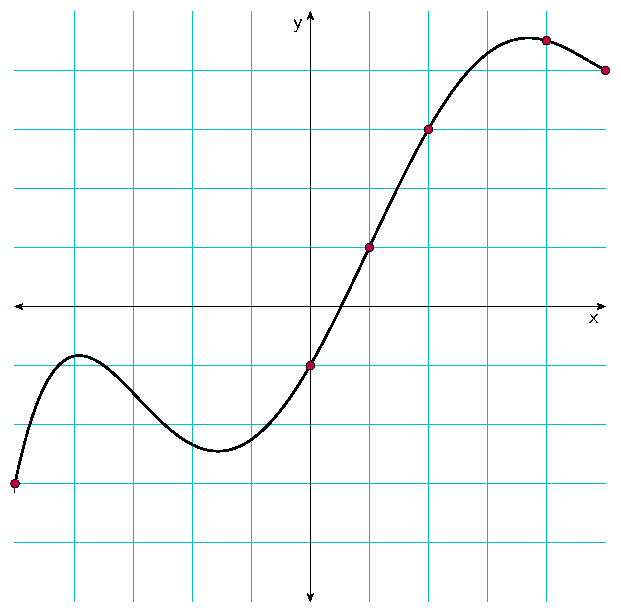
\includegraphics[scale=0.75]{figures/lagrange_poly_plot1.pdf}
\caption{Plot of a Lagrange Polynomial}
\label{fig:lagrange_poly_plot1}
\end{figure}

\hyperref[fig:lagrange_poly_plot1]{Figure \ref{fig:lagrange_poly_plot1}} shows the Lagrange polynomial going through 
the points, 
\[ \left\{(1,1), (2,3), (0, -1), (5, 4), (-5, -3), (4, 4.5) \right\}\] 
We can easily compute Lagrange polynomials in python using \texttt{sympy}.

\begin{mdcode}
\begin{minted}[mathescape, breaklines, ]{pycon}
>>> import sympy
>>> x = sympy.symbols('x')
>>> points = [(1,1), (2,3), (0, -1), (5, 4), (-5, -3), (4, 4.5)]
>>> expr = sympy.interpolate(points, x)
>>> print(expr)
0.00281746031746032*x**5 - 0.0129761904761905*x**4 - 0.111944444444445*x**3 + 0.384404761904762*x**2 + 1.73769841269841*x - 1
\end{minted}
\end{mdcode}

\begin{problem}
    Let $P(x)$ be a polynomial of degree $n$ such that, $P(k)=2^{k}$ for all $0\leq k \leq n$. Find $P(n+1)$.
\end{problem}
\begin{sol}
    From \hyperref[thm:lagrange-interpol]{Theorem \ref{thm:lagrange-interpol}} we have,
    \begin{align*}
        P(x) = \sum_{k=0}^{n} 2^{k}D_{k}(x)
    \end{align*}
    where,
    \begin{align*}
        D_{k}(x) &= \frac{x(x-1)\cdots (x-k+1)(x-k-1)(x-k-2)\cdots (x-n+1)(x-n)}{(k)(k-1)\cdots (1)(-1)(-2) \cdots (k-n+1)(k-n)} \\
        &= (-1)^{n-k} \frac{x(x-1)\cdots (x-k+1)(x-k-1)(x-k-2)\cdots (x-n+1)(x-n)}{k!(n-k)!}
    \end{align*}
    Therefore,
    \begin{align*}
        P(n+1) &= \sum_{k=0}^{n} (-1)^{n-k} 2^{k} \frac{(n+1)n(n-1)\cdots (n-k+2)(n-k)(n-k-1)\cdots 1}{k!(n-k)!} \\
               &= \sum_{k=0}^{n} (-1)^{n-k} 2^{k} \frac{(n+1)!}{k!(n-k)!(n-k+1)} \\
               &= \sum_{k=0}^{n} (-1)^{n-k} 2^{k} {n+1 \choose k} \\
               &= (-1) \left( \sum_{k=0}^{n+1} {n+1 \choose k} 2^{k} (-1)^{n-k+1} \right) + 2^{n+1} \\
               &= (-1)\left( 2 - 1 \right)^{n+1} + 2^{n+1} \\
               &= 2^{n+1} - 1
    \end{align*}    
\end{sol}
\end{document}
